\documentclass[color,t,presentation,english,aspectratio=169]{beamer}



\usetheme[
% insert a header below title showing the sections (short section names) for navigation,
	%secheader,
	%
% insert a header above title showing current chapter ou section 
	%currentsecheader,
	%
% text is in english, default is french
	isinenglish,
	%
% print outline at beginning section, default is false	
	outlineabs,
	%
% print partner's log: ubl, ccbyncsa, cnrs, subatech, irisa, inserm, lab-sticc, marsouin, ls2n, gepea, ubl, loustic, ifremer
% TO DO: lego, atol, latim, cominglab, etc.
	secondlogo=ccbyncsa,
	%
% print notes, default is false	
	%printnotes,
	%
% slides per page: 1 (default), 2, 4 --landscape--	
	slidesparpage=1,
	%
% section or chapter in headline, default chapter	
	sectorchapt=section, %section
	%
% Add a footline with title and author
	% footline,
	%
	]
{IMTAtlantique}




\usepackage[utf8]{inputenc}
\usepackage[english]{babel} 
%\usepackage[latin1]{inputenc}
\usepackage{xspace}
\usepackage{amssymb}
%\usepackage{amsmath}
\usepackage{graphicx}
\usepackage{color}
\usepackage{xcolor}
\usepackage{multirow}
\usepackage{rotating}
\usepackage{array}%
\usepackage{fancybox}
\usepackage{hhline}
\usepackage{tikz}
\usetikzlibrary{calc,arrows,shapes,decorations}
\usepackage{xifthen}
\usepackage{bbm}
\usepackage[absolute]{textpos}

\usepackage{booktabs}

\usepackage{pgfpages}
\usepackage{format-IMT-Atlantique}

%
% Properly spaced abbreviations
% Taken from the CVPR's style package (https://stackoverflow.com/a/39363004)
%
\usepackage{xspace}

% Add a period to the end of an abbreviation unless there's one
% already, then \xspace.
\makeatletter
\DeclareRobustCommand\onedot{\futurelet\@let@token\@onedot}
\def\@onedot{\ifx\@let@token.\else.\null\fi\xspace}
%
\def\eg{\emph{e.g}\onedot} \def\Eg{\emph{E.g}\onedot}
\def\ie{\emph{i.e}\onedot} \def\Ie{\emph{I.e}\onedot}
\def\cf{\emph{c.f}\onedot} \def\Cf{\emph{C.f}\onedot}
\def\etc{\emph{etc}\onedot} \def\vs{\emph{vs}\onedot}
\def\wrt{w.r.t\onedot} \def\dof{d.o.f\onedot}
\def\etal{\emph{et al}\onedot}
\makeatother



\usepackage{fontspec}
\setmainfont{Arial}

\setbeamertemplate{section in head/foot shaded}[default][75]
\setbeamertemplate{section in head/foot shaded}[default][25]


\usepackage[acronym]{glossaries}
\glsdisablehyper
\loadglsentries{glossary}
\makenoidxglossaries


\usepackage{layouts}
\usepackage{printlen}
\usepackage{verbatim}

\makeatletter
\newcommand{\printfontsize}[1]{{#1\the\dimexpr\f@size pt\relax}}
\makeatother

\usepackage[style=ieee]{biblatex}
\addbibresource{references.bib}
\addbibresource{own.bib}
\renewcommand*{\bibfont}{\scriptsize}

\title{\vspace{3\baselineskip}What if the attackers are inside?\\}

\subtitle{A Systematic Analysis of Label-flipping Attacks against Federated Learning for Intrusion Detection\\\linebreak}

\author{\underline{\textbf{Léo Lavaur}}\textsuperscript{1}, Yann Busnel\textsuperscript{2}, and Fabien Autrel\textsuperscript{1}}

\institute{\textsuperscript{1} IMT Atlantique, \textsuperscript{2} IMT Nord Europe\\}
    

\date{\scriptsize 4th International Workshop on Behavioral Analysis for System Security\\ co-located with the ARES conference, August 2, 2024}

\begin{document}

\maketitle

\begin{frame}
	\frametitle{\acrfull{nids}}
	\glsunset{nids}

	\begin{figure}
		\centering
		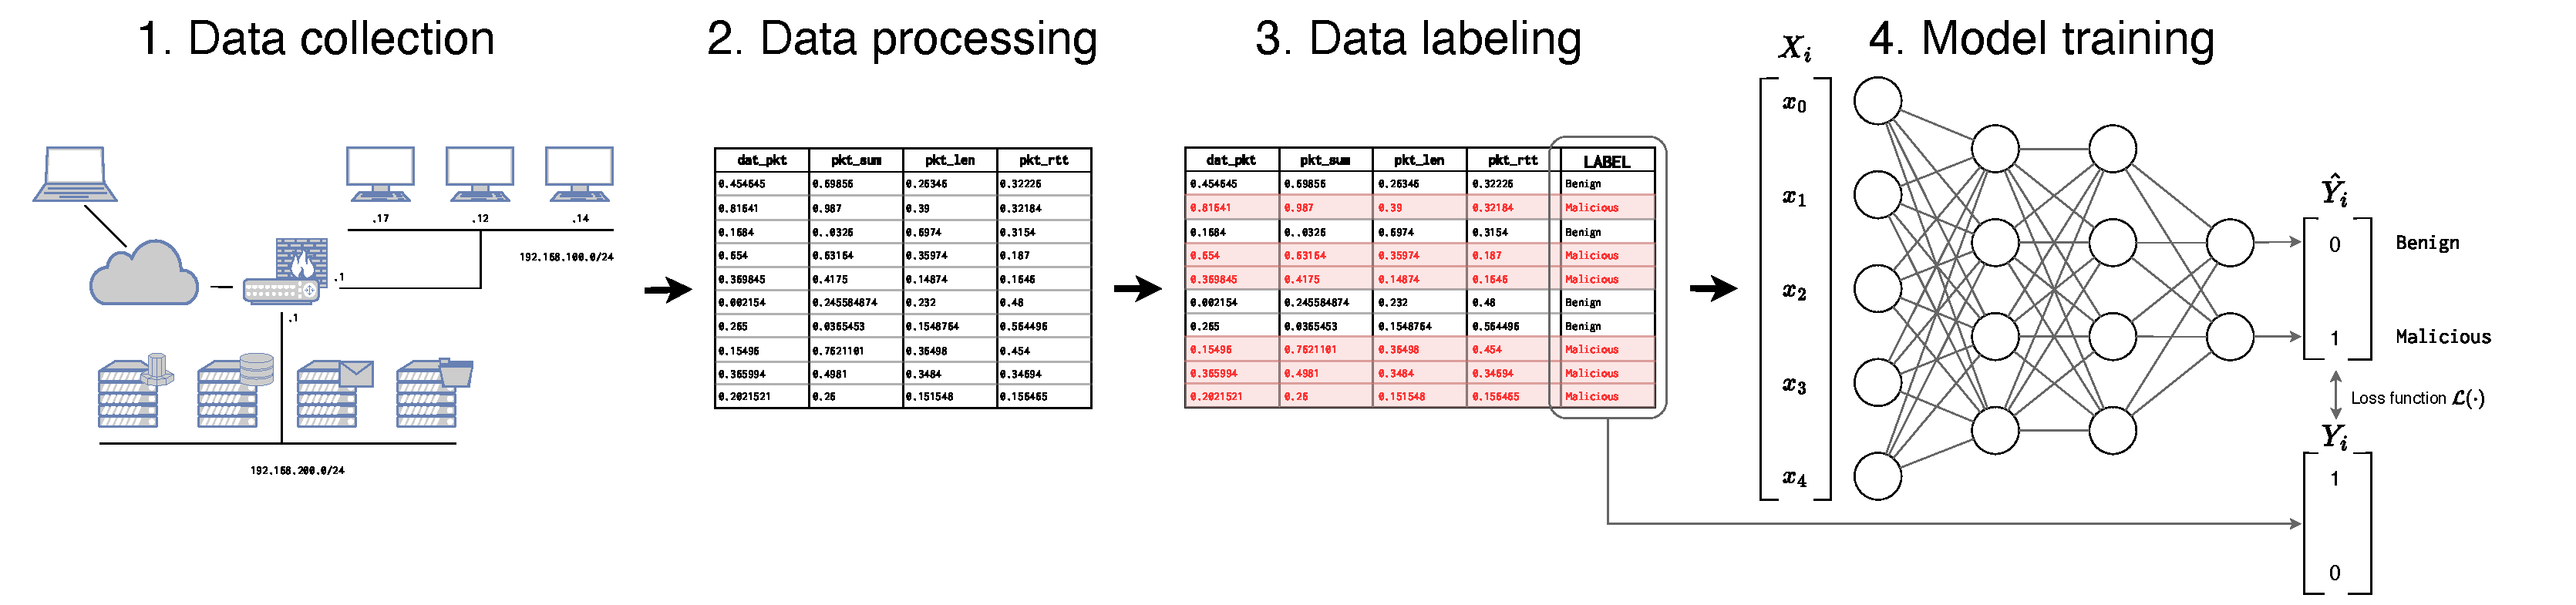
\includegraphics[width=\linewidth]{./figures/mlp-workflow.pdf}
		\caption{Typical \acrshort{nids} workflow.}
	\end{figure}

	\begin{itemize}
		\item Great performance with \Gls{dl} (on public datasets at least)
		\item \textbf{Limitations}: lack of labelled data, risk of local bias or skewed data distribution, inefficient against new attacks.
	\end{itemize}

\end{frame}

\begin{frame}
	\frametitle{Scaling~\gls{nids} with \acrshort{fl}}

	\begin{columns}
		\begin{column}{0.4\linewidth}
			\vspace{-\textheight}
			\begin{itemize}
				\item \Acrfull{fl} is a distributed \Acrfull{ml} paradigm~\cite{mcmahan_Communicationefficientlearningdeep_2017}.
				\item Participants train a global model without sharing local data.
			\end{itemize}
		\end{column}
		\begin{column}{0.6\linewidth}
			\begin{overlayarea}{\linewidth}{\textheight}
				\only<1>{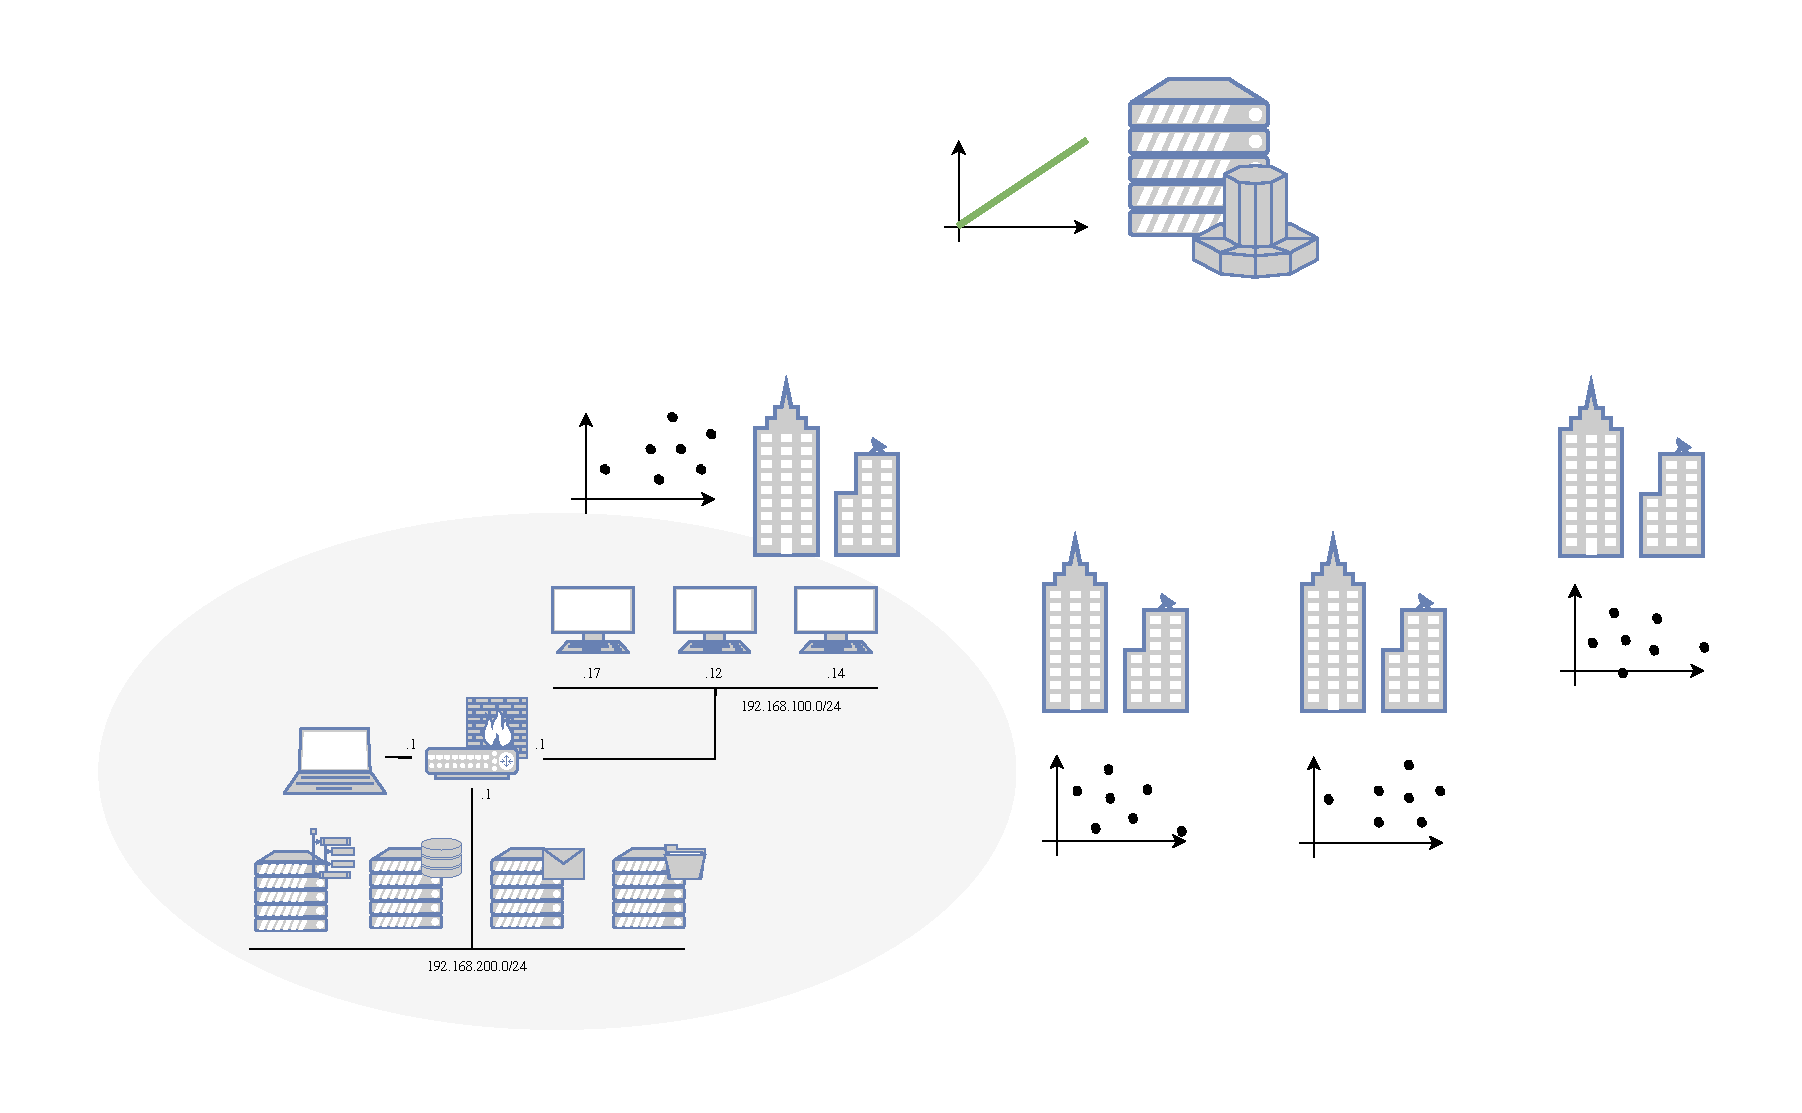
\includegraphics[width=\linewidth]{./figures/fl-1.pdf}}
				\only<2>{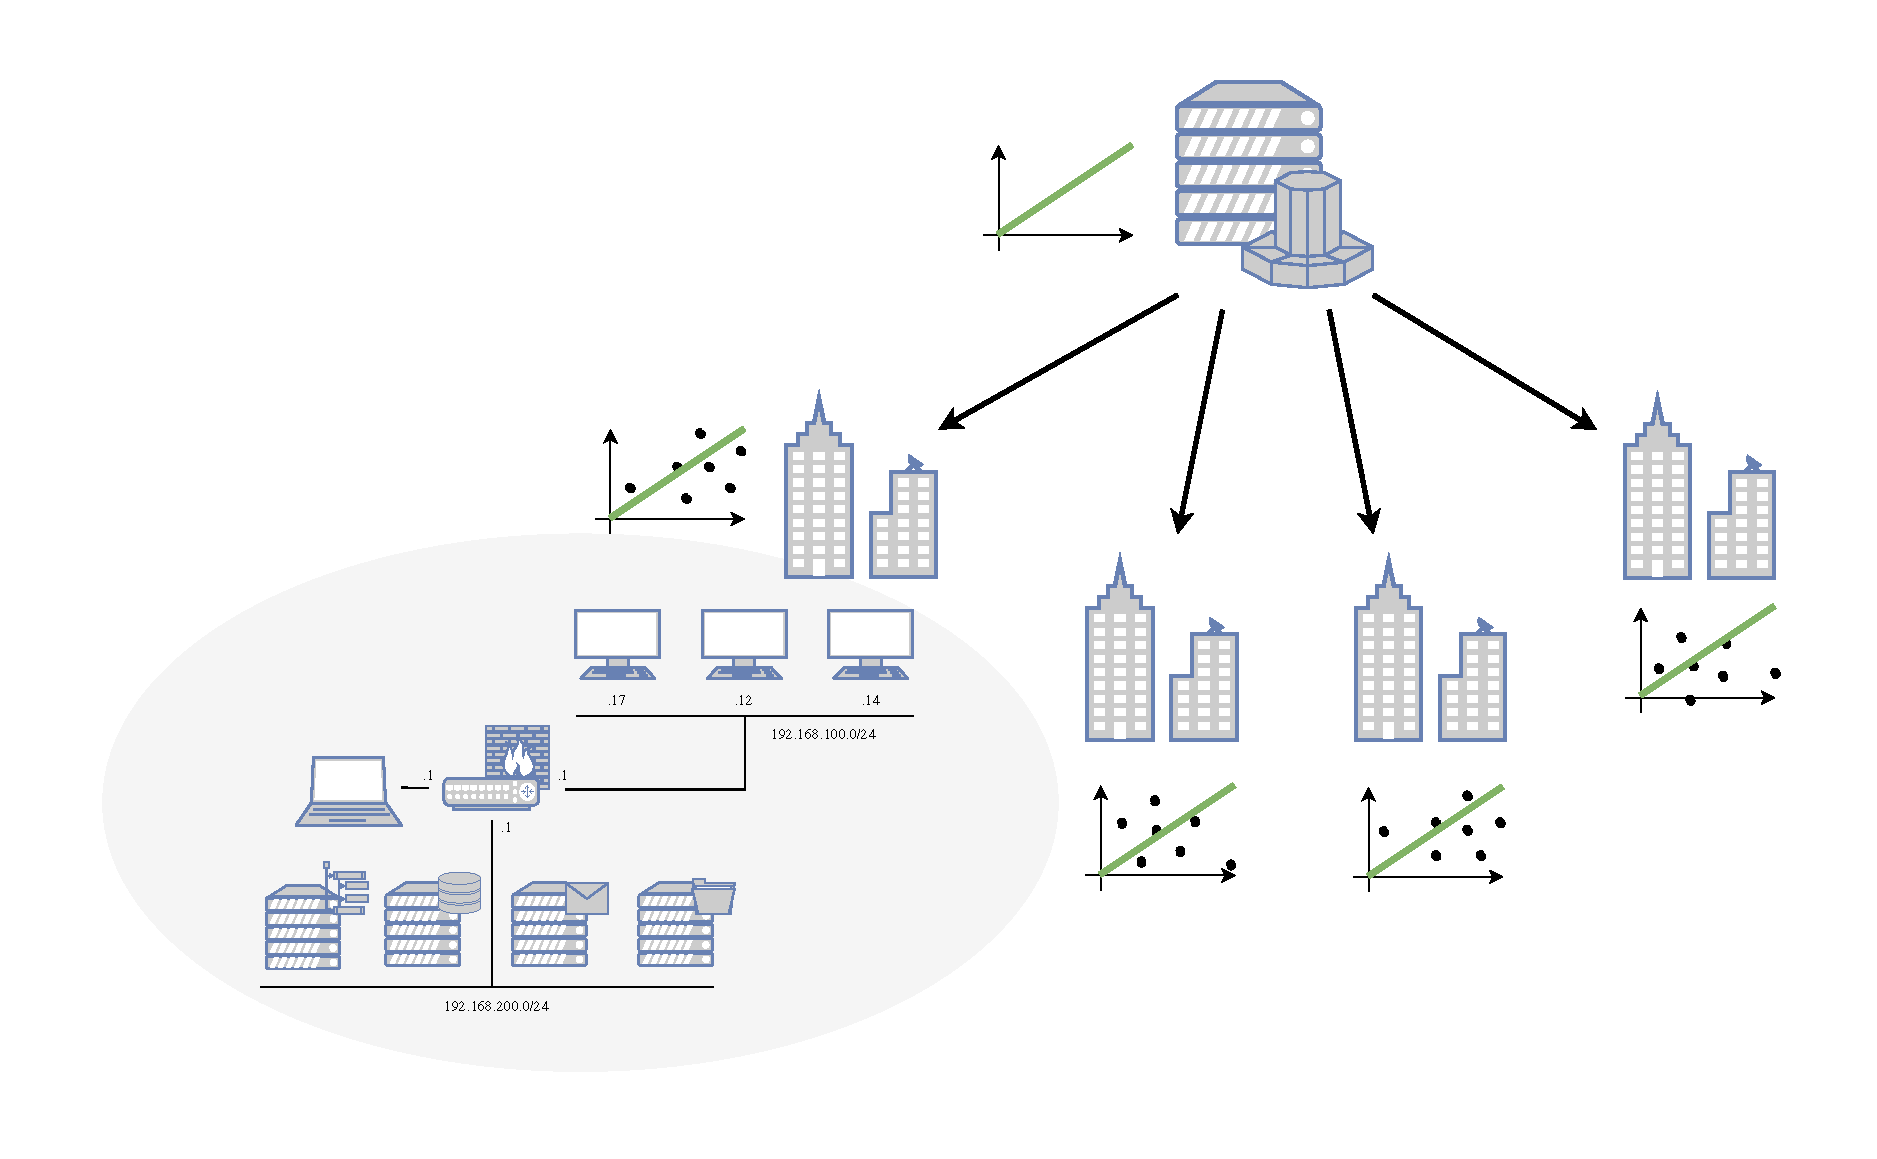
\includegraphics[width=\linewidth]{./figures/fl-2.pdf}}
				\only<3>{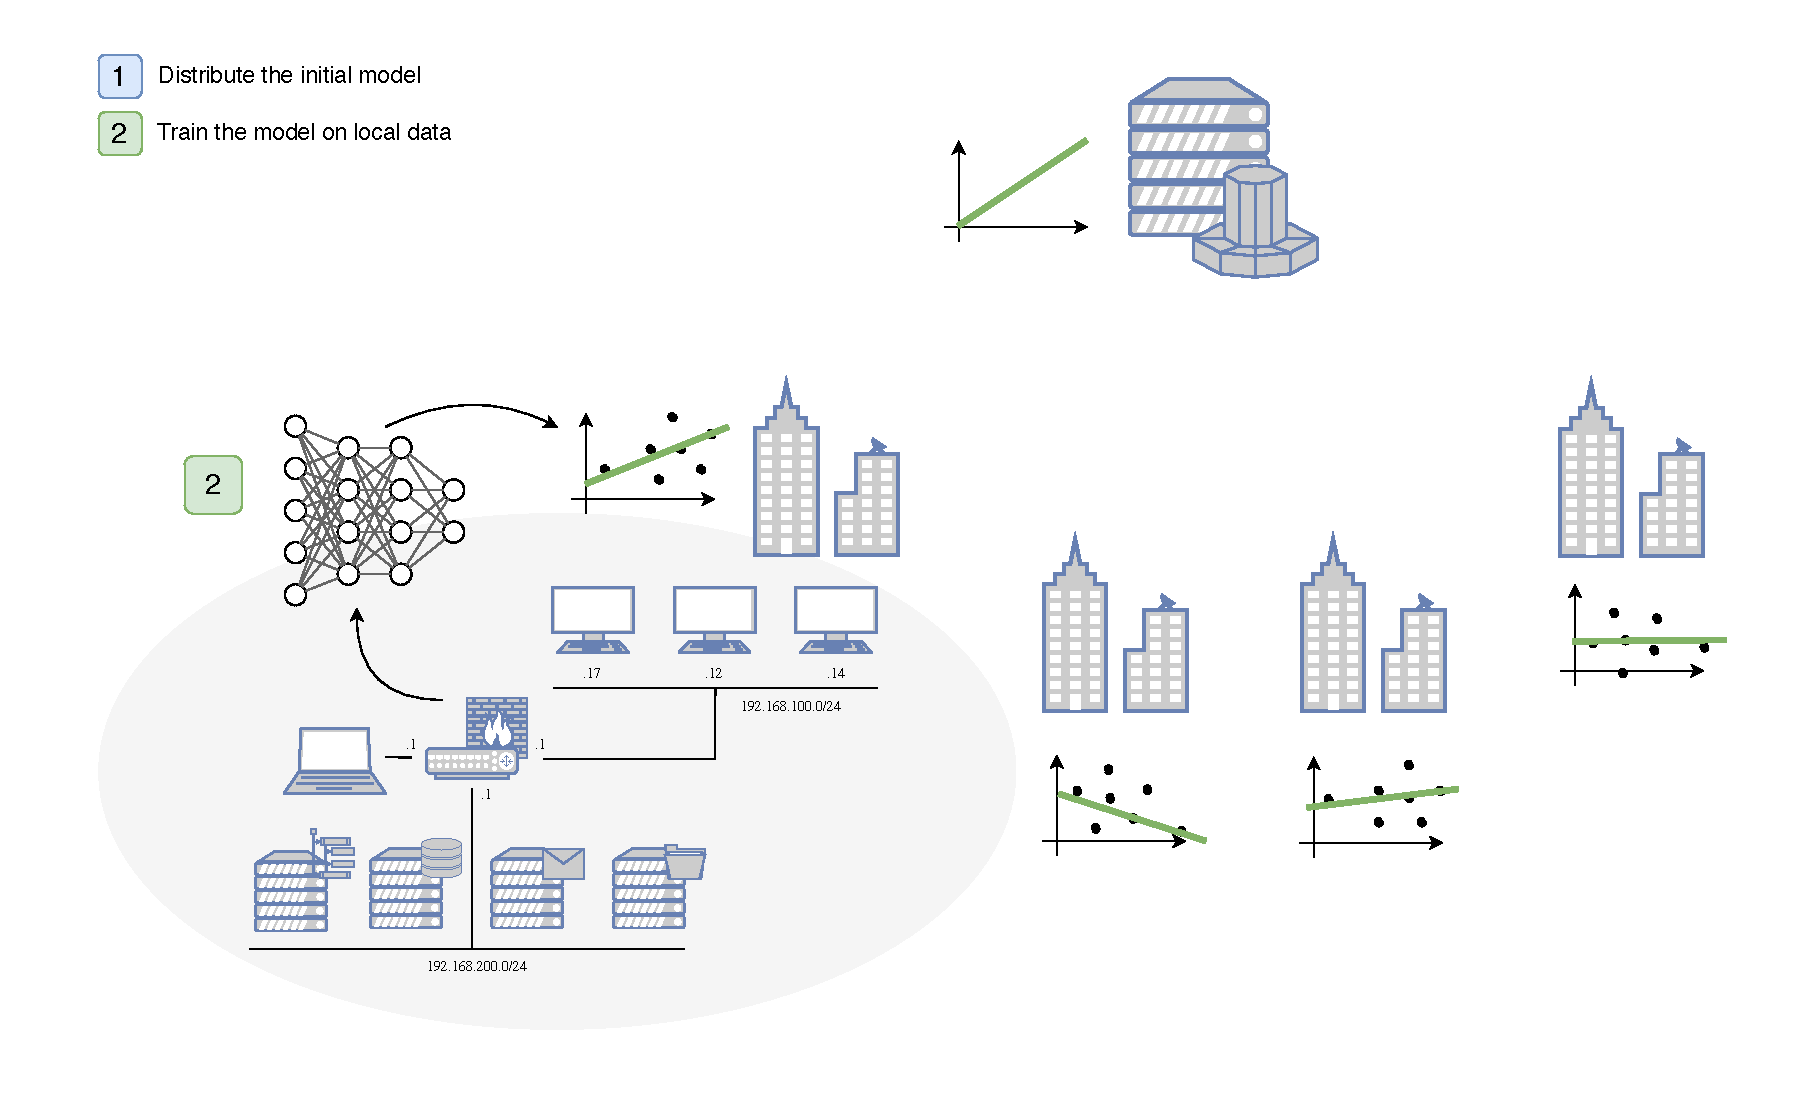
\includegraphics[width=\linewidth]{./figures/fl-3.pdf}}
				\only<4>{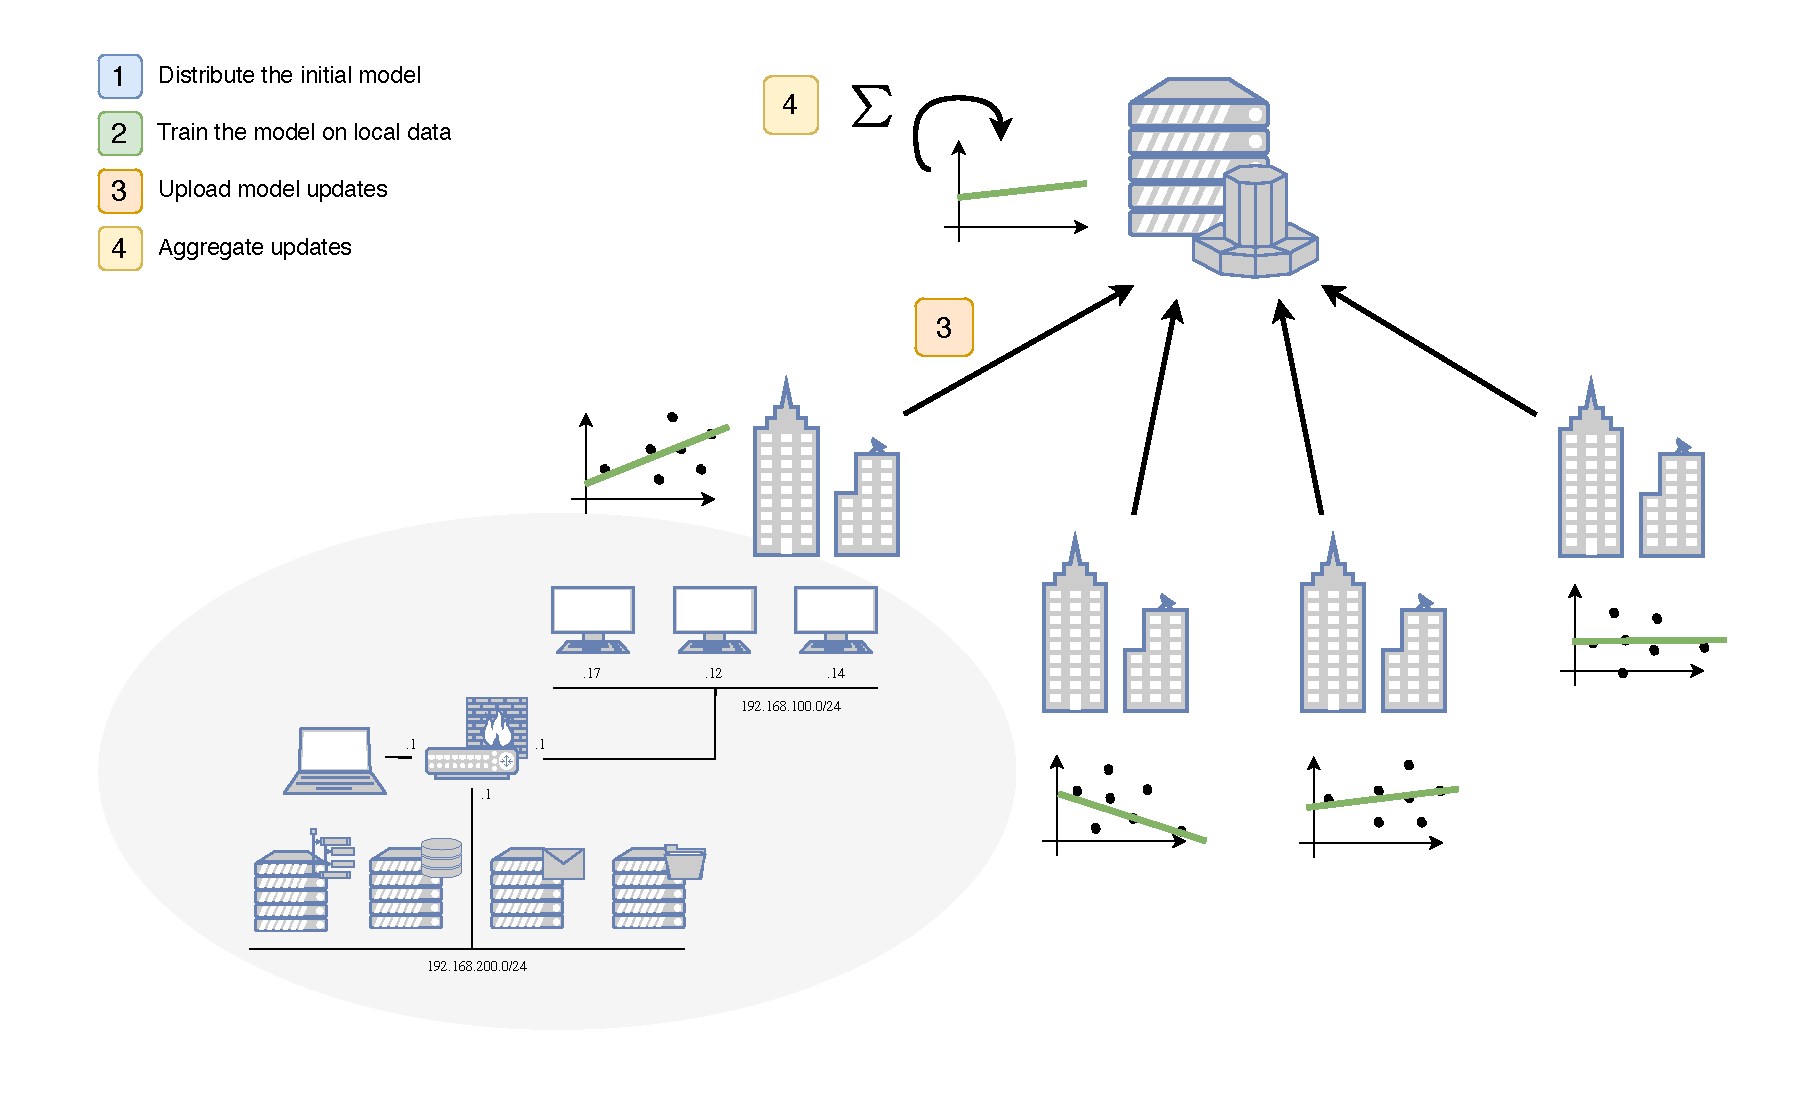
\includegraphics[width=\linewidth]{./figures/fl-4.pdf}}
				\only<5>{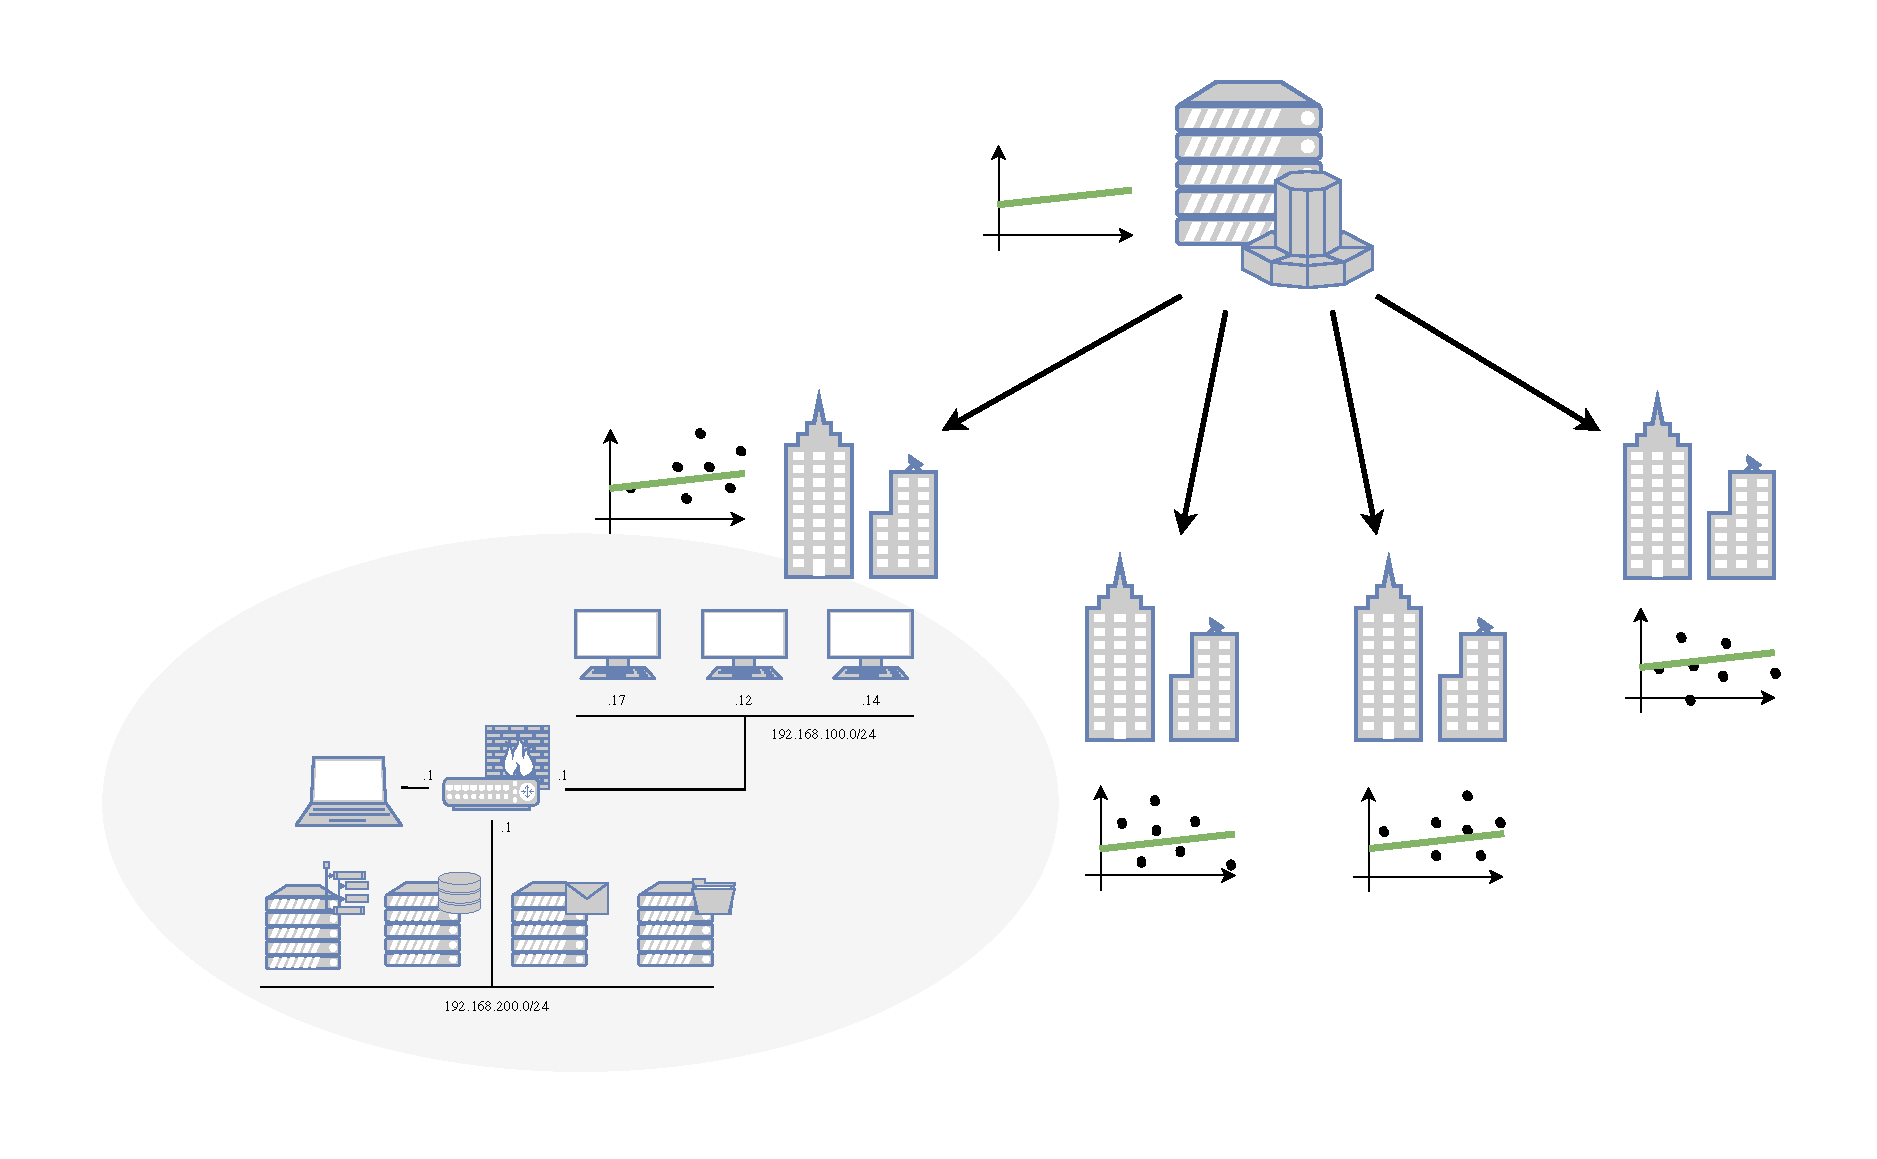
\includegraphics[width=\linewidth]{./figures/fl-5.pdf}}
			\end{overlayarea}
		\end{column}
	\end{columns}
\end{frame}

\glsunset{fids}
\glsunset{fl}
\glsunset{ml}

\begin{frame}
	\frametitle{\acrfull{fids}}
	\begin{columns}
		\begin{column}{0.5\linewidth}
			\begin{overlayarea}{\linewidth}{\textheight}
				\vspace{.5ex}
				FL can be used in \Acrfull{cids}~\cite{lavaur_tnsm_2022}:
				\begin{itemize}
					\item Extend the training data with \acrfull{hfl}
					\begin{itemize}
						\item[$\rightarrow$] Reduce the risk of local bias
					\end{itemize}
					\only<2>{\item Effectively share knowledge (\eg, on specific classes, instances) between participants
					\begin{itemize}
						\item[$\rightarrow$] Share the knowledge about a new attack~\cite{lavaur_icdcs_demo_2024};
						\item[$\rightarrow$] Improve the characterization of specific devices; \dots
					\end{itemize}}
				\end{itemize}
			\end{overlayarea}
		\end{column}
		\begin{column}{0.5\linewidth}
			\vspace{-.8\textheight}
			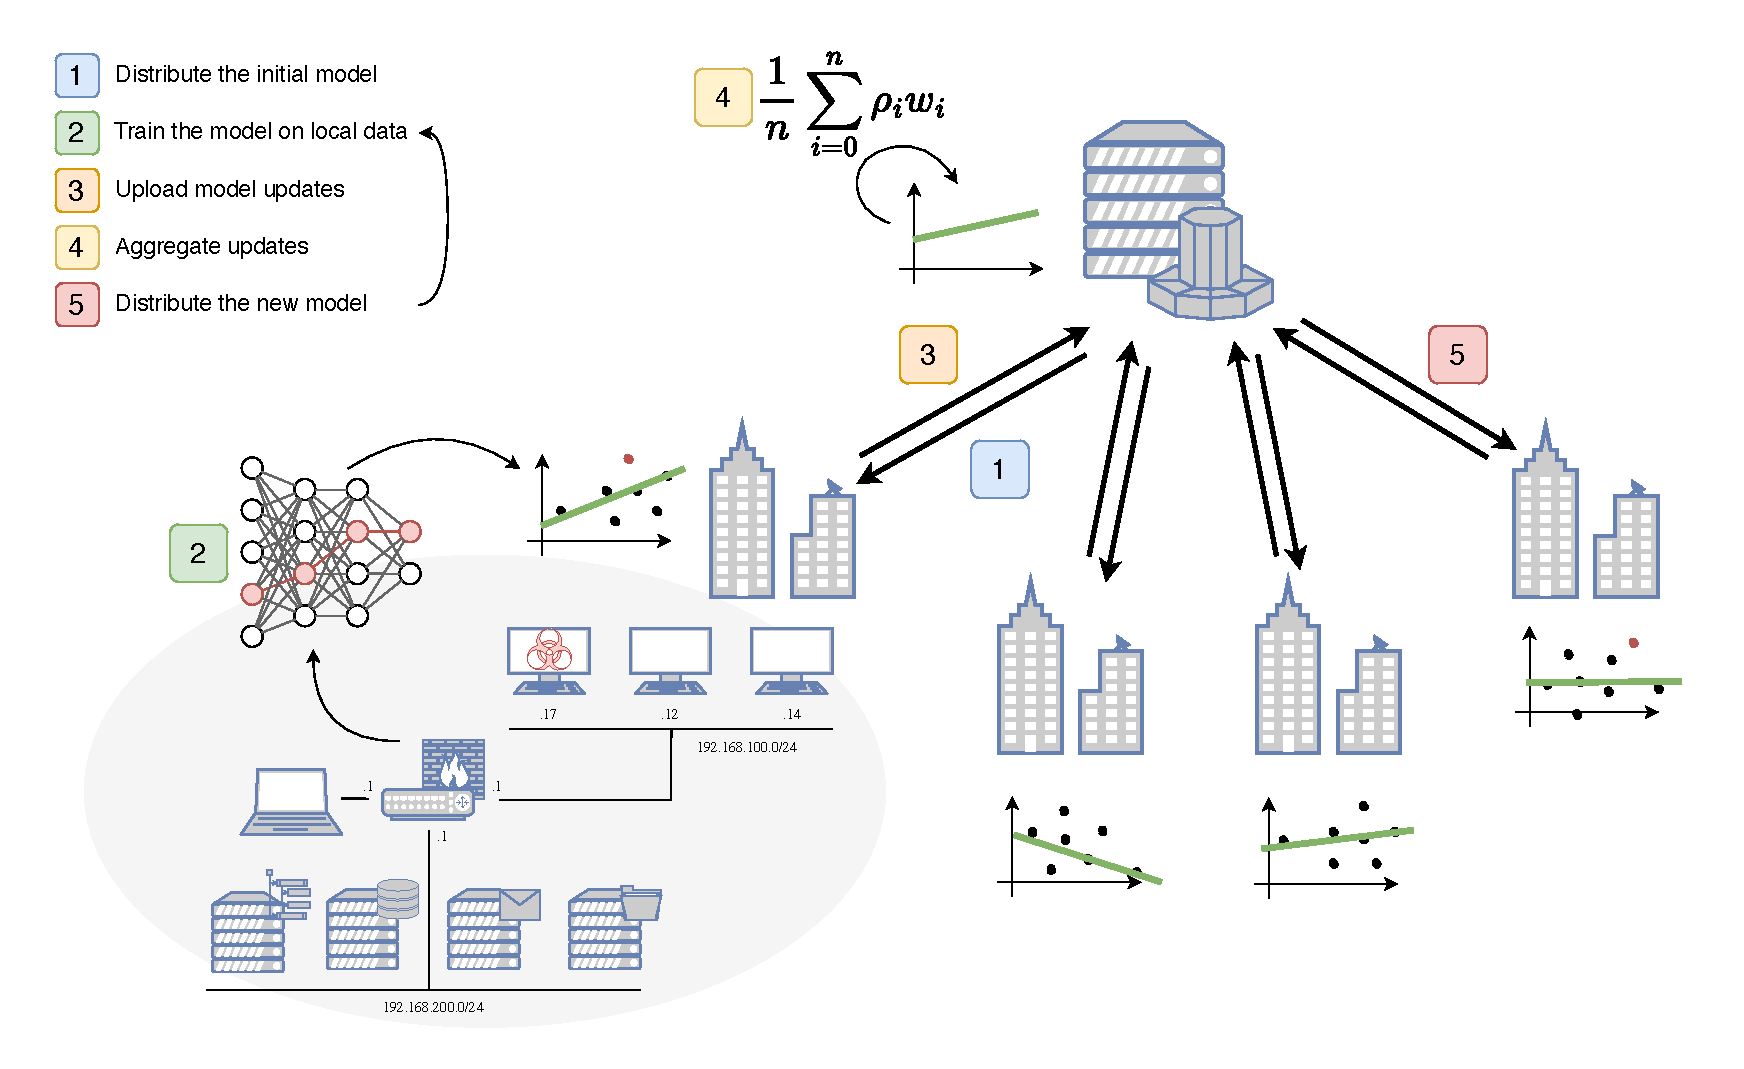
\includegraphics[width=\linewidth]{./figures/fl.pdf}
		\end{column}
	\end{columns}
\end{frame}

\glsunset{hfl}

\begin{frame}
	\frametitle{\Gls{fl} against malicious contributions}

	\begin{columns}
		\begin{column}{0.4\linewidth}
			\vspace{-\textheight}
			\begin{itemize}
				\item \Gls{fl} is highly susceptible to poisoning~\cite{tolpegin_DataPoisoningAttacks_2020}.
				\only<6>{%
					\item The impact is difficult to estimate.
					\begin{itemize}
						\item Few studies in the \gls{fids} context, often partial.
						\item Nothing on aggregated classes.
					\end{itemize}%
				}
			\end{itemize}
		\end{column}
		\begin{column}{0.6\linewidth}
			\begin{overlayarea}{\linewidth}{\textheight}
				\only<1>{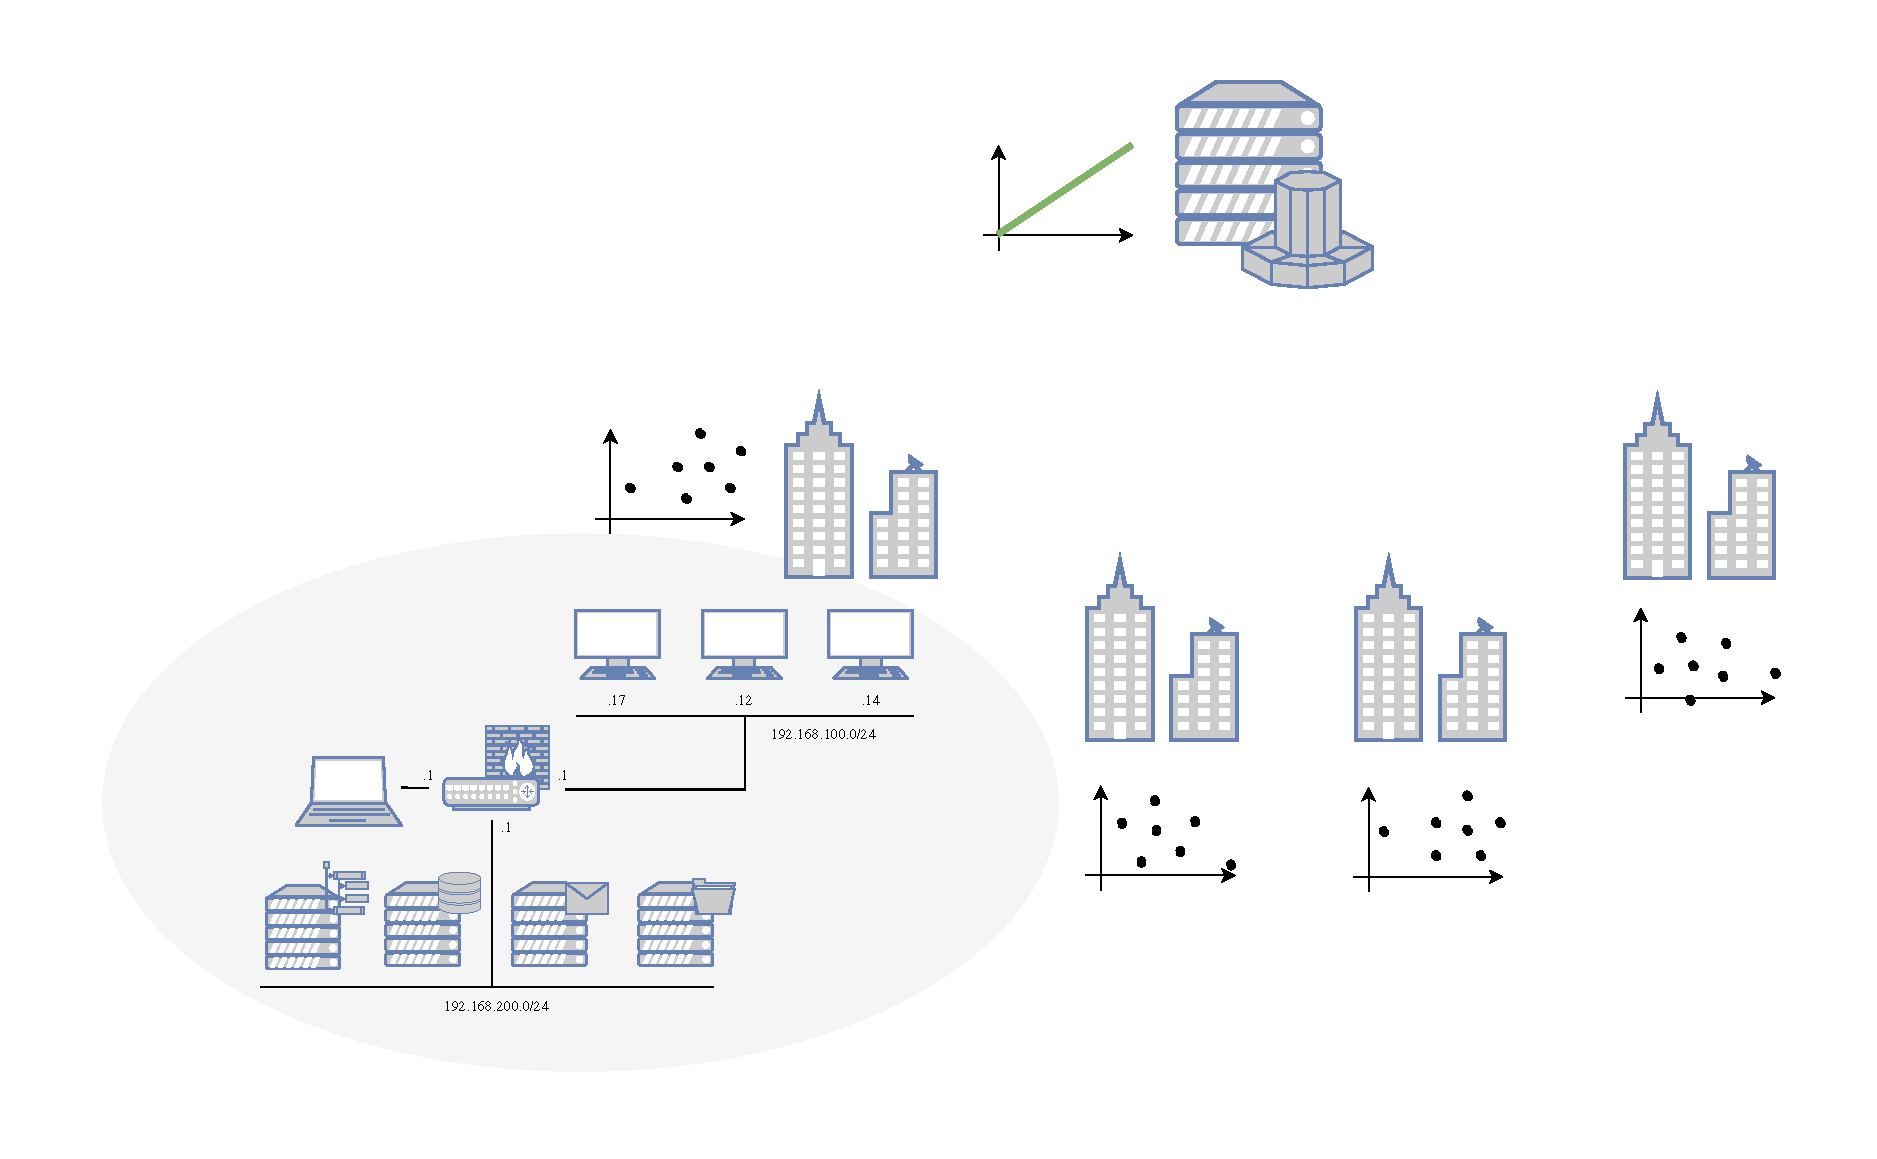
\includegraphics[width=\linewidth]{./figures/fl-poisoning-1.pdf}}
				\only<2>{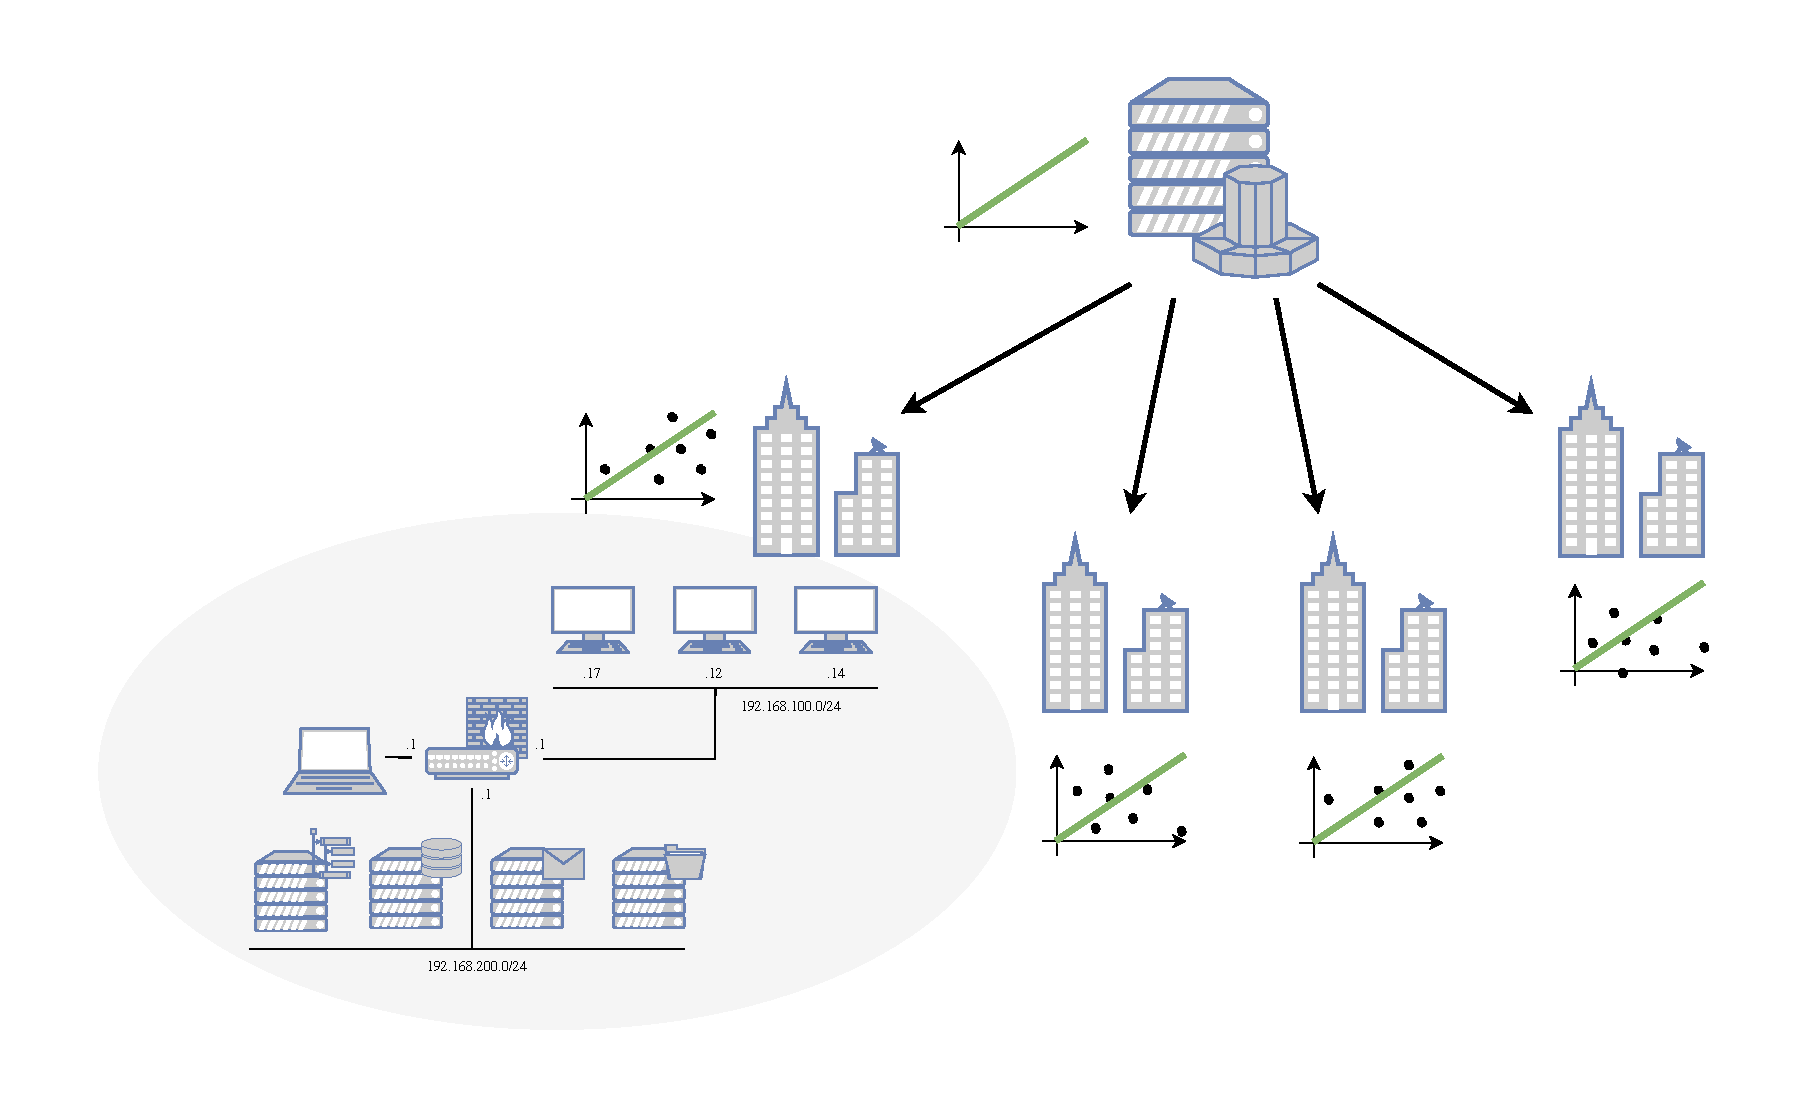
\includegraphics[width=\linewidth]{./figures/fl-poisoning-2.pdf}}
				\only<3>{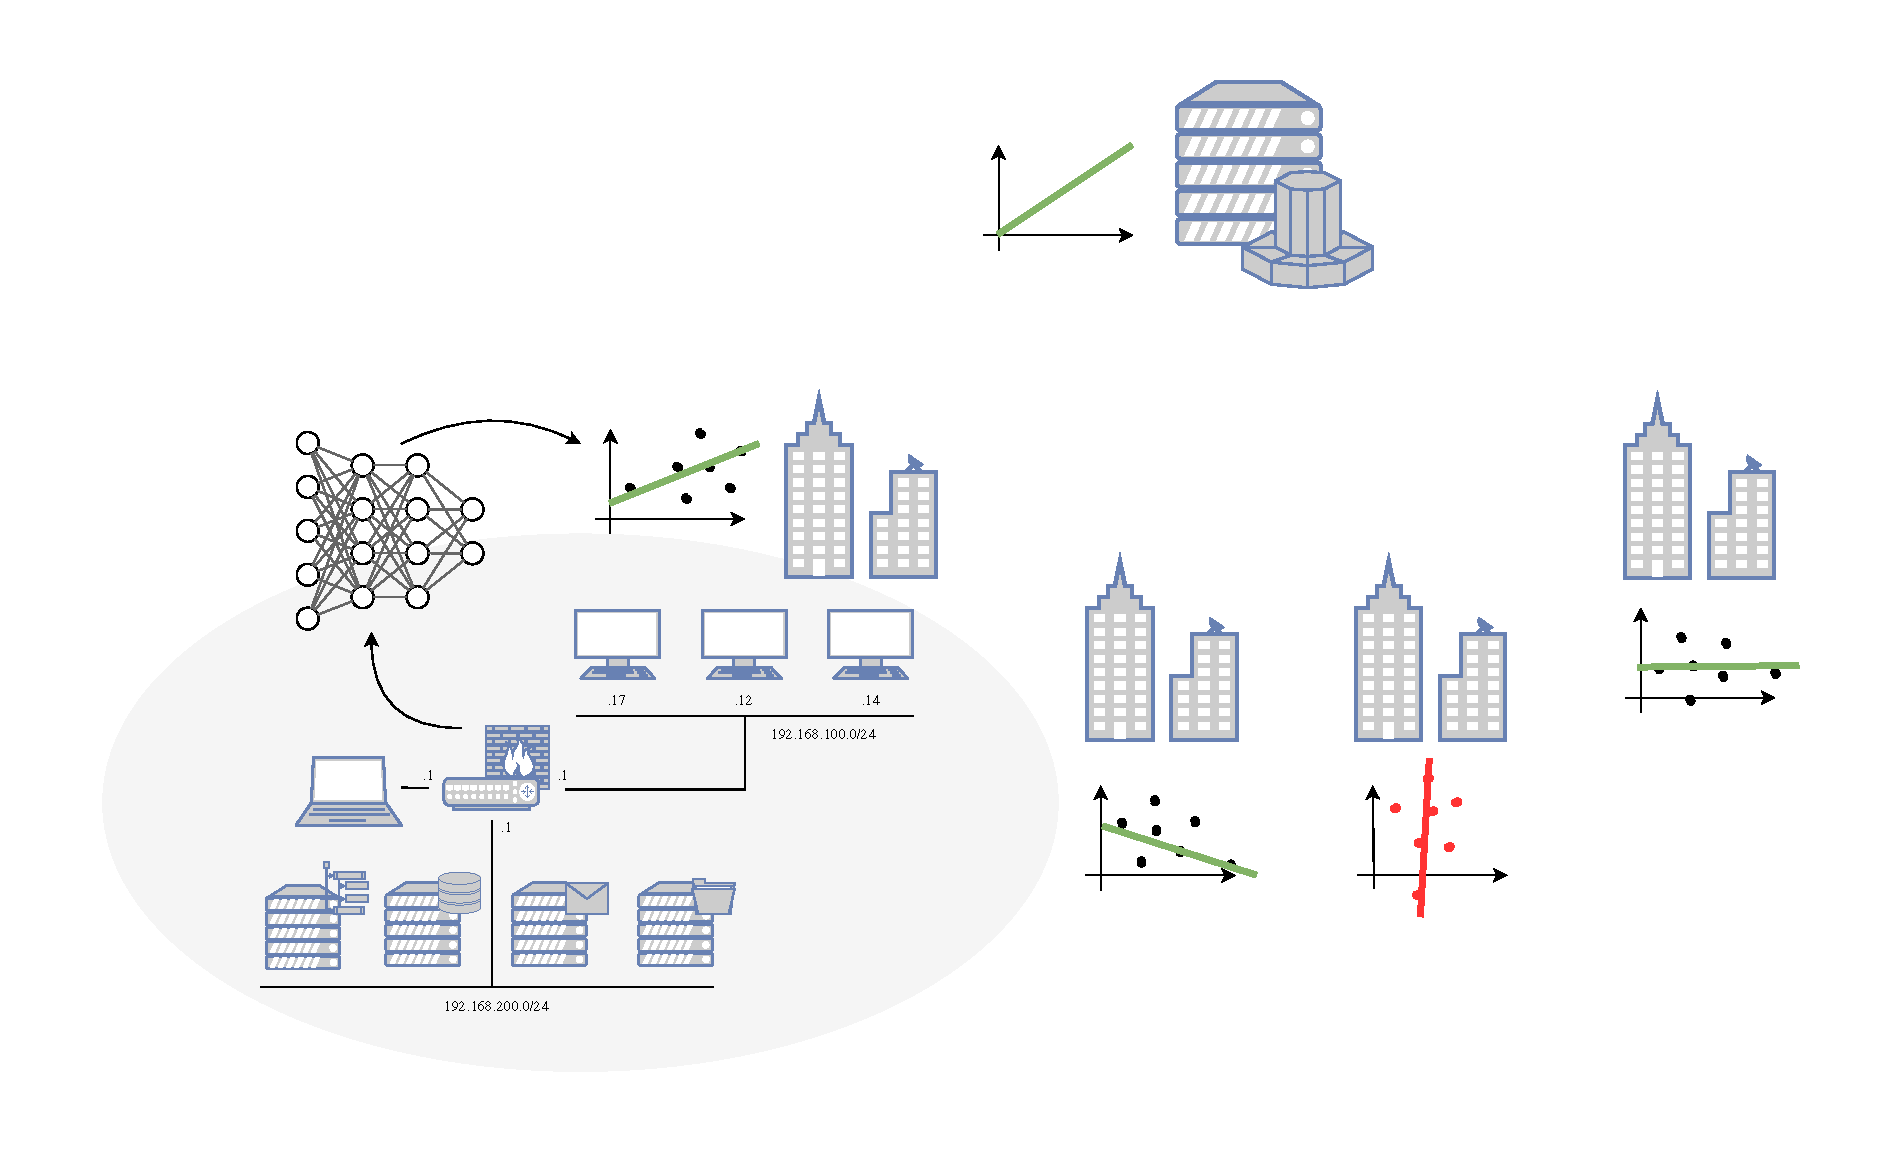
\includegraphics[width=\linewidth]{./figures/fl-poisoning-3.pdf}}
				\only<4>{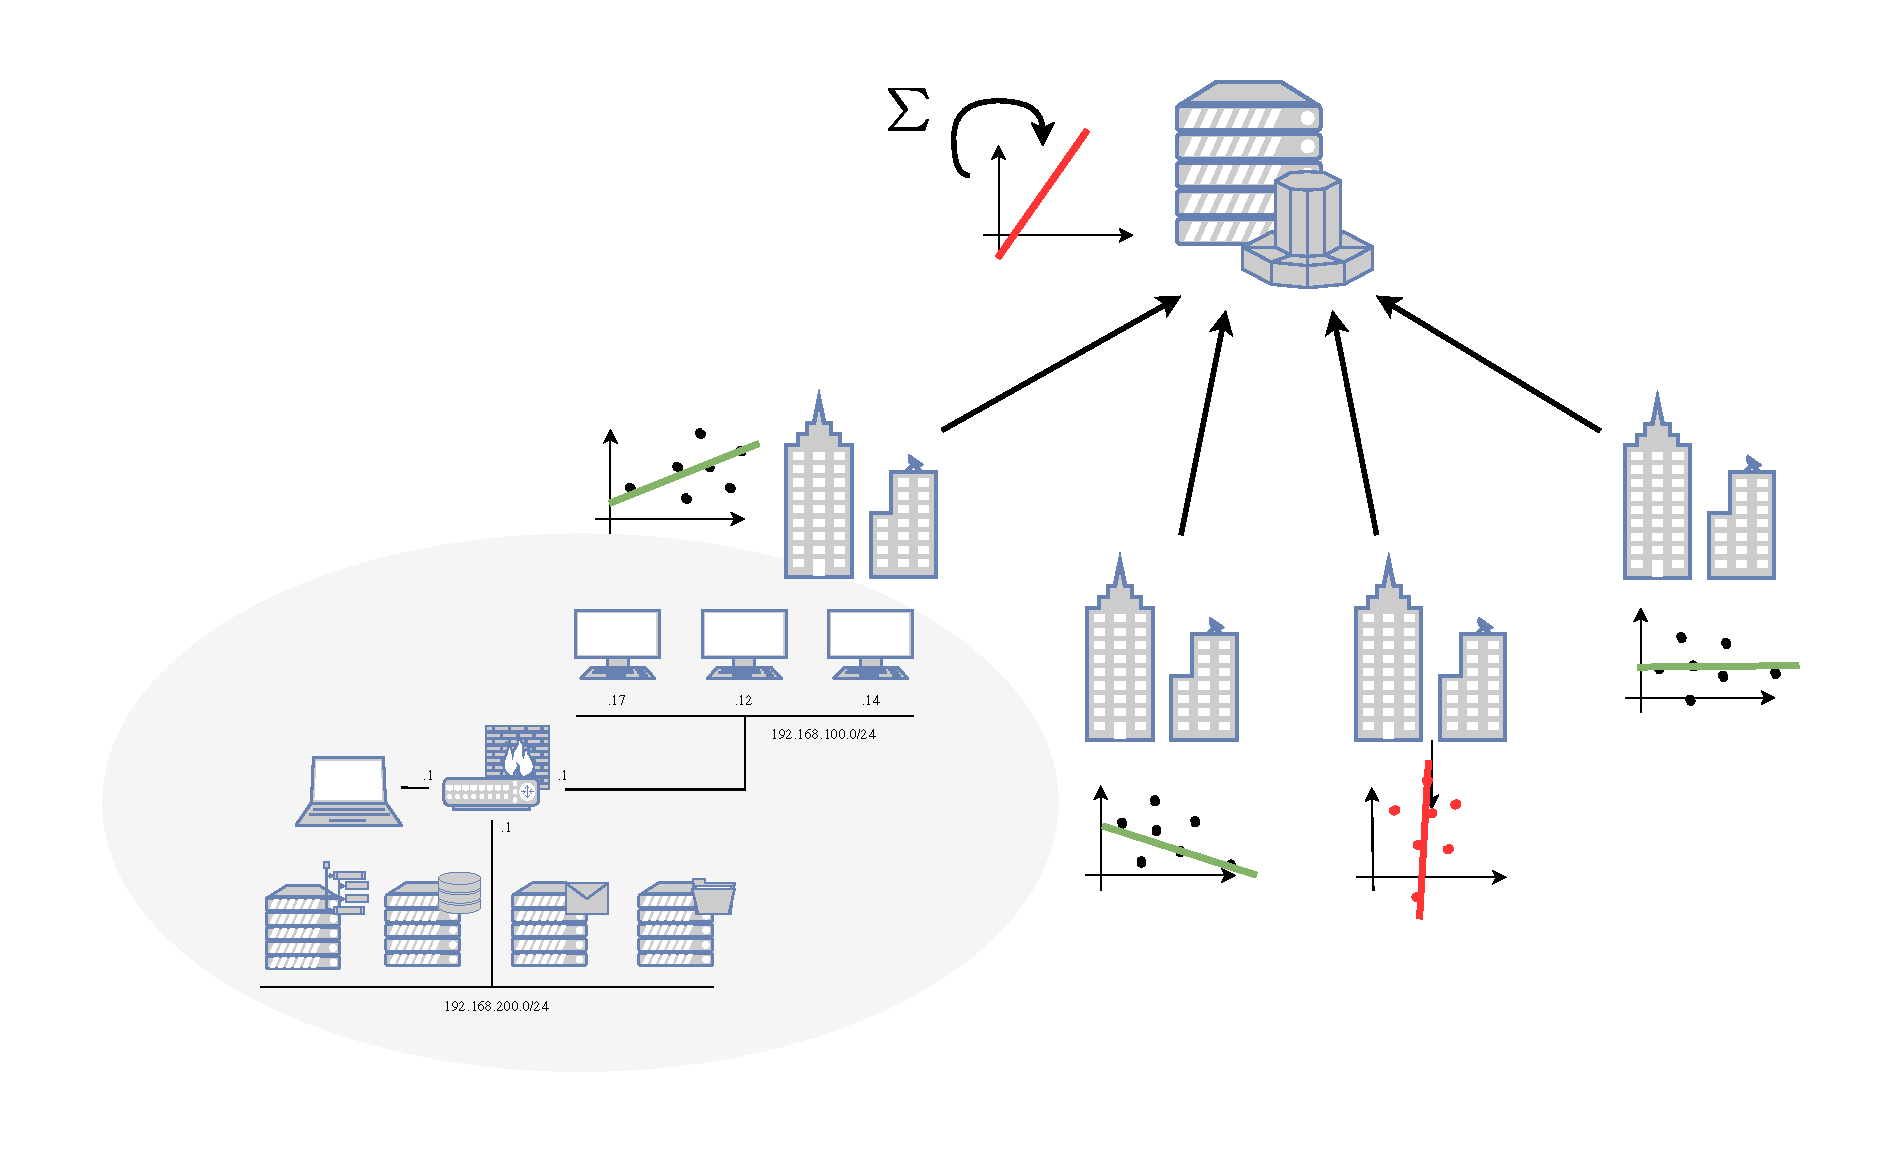
\includegraphics[width=\linewidth]{./figures/fl-poisoning-4.pdf}}
				\only<5->{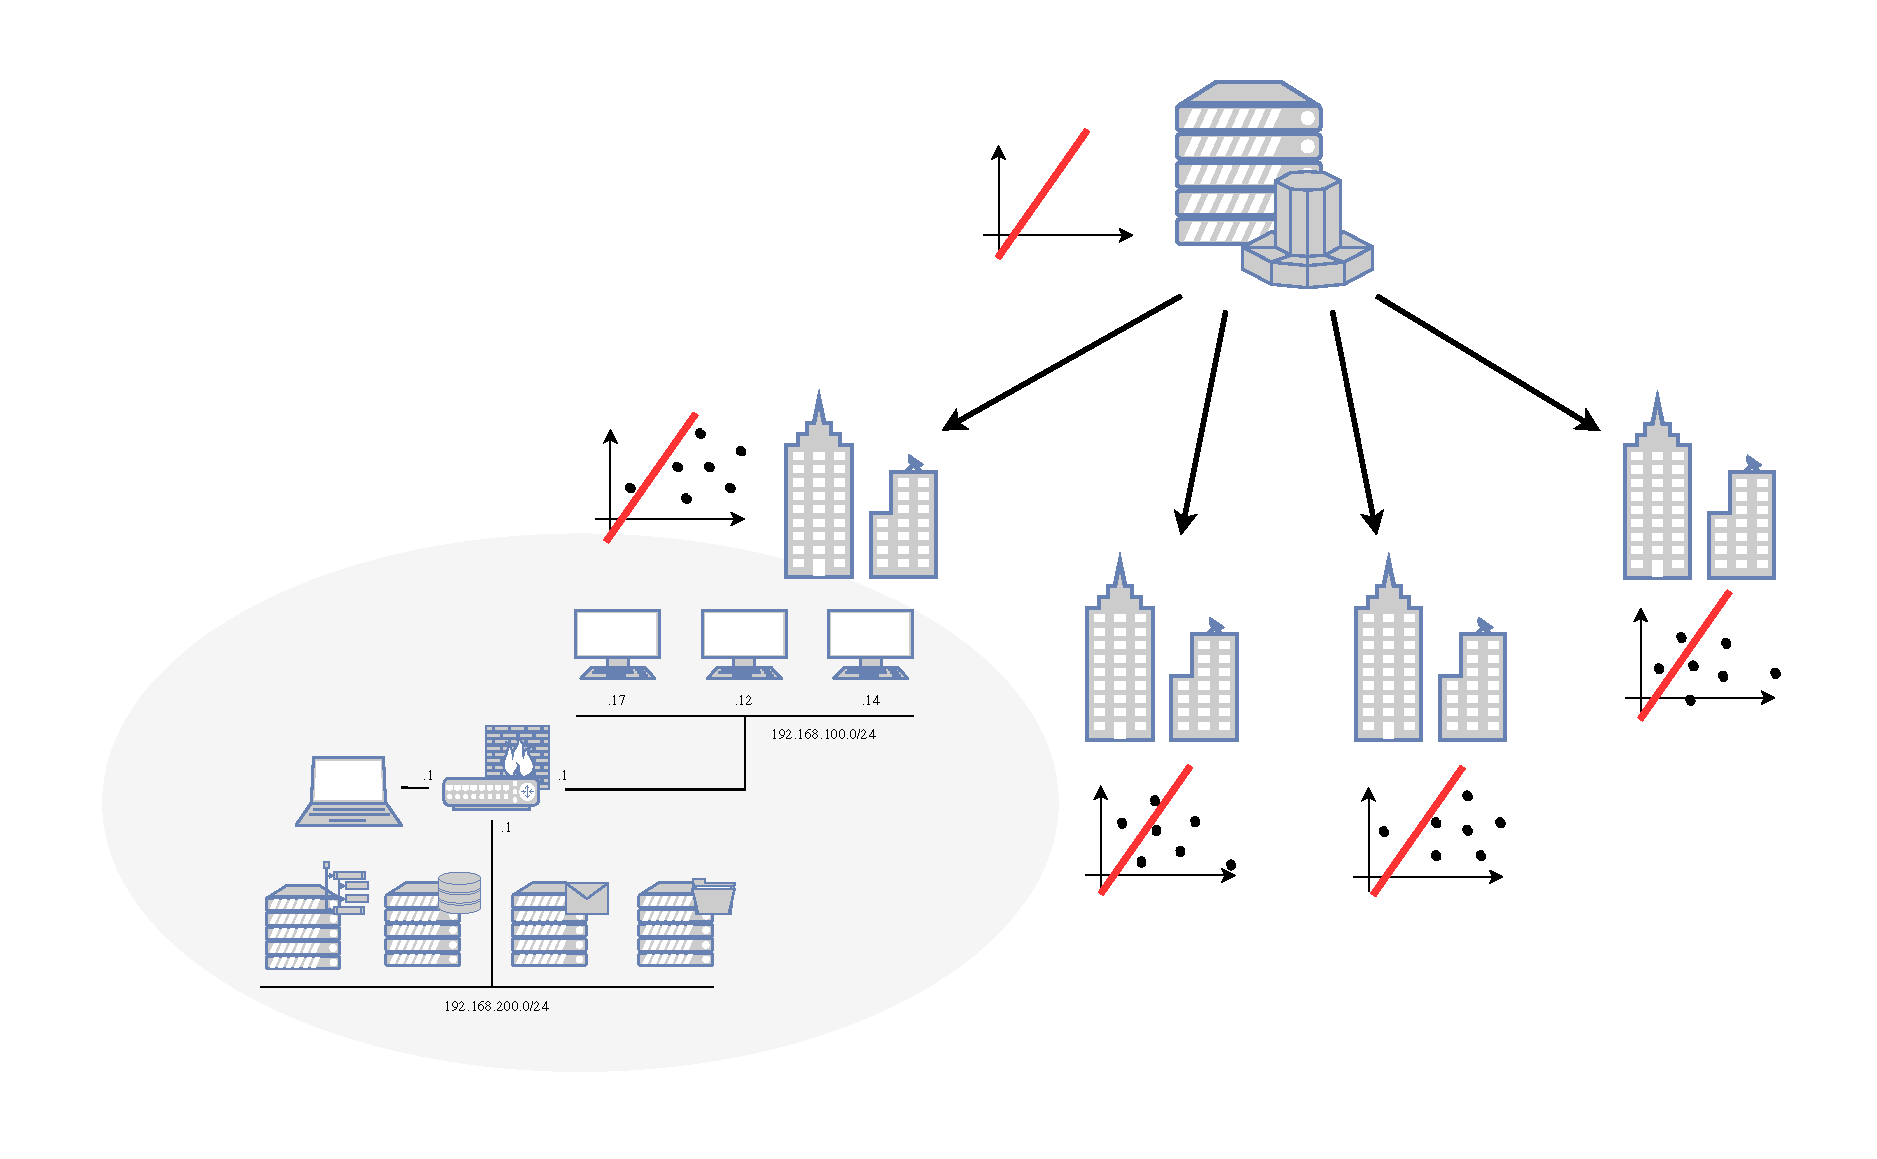
\includegraphics[width=\linewidth]{./figures/fl-poisoning-5.pdf}}
			\end{overlayarea}
		\end{column}
	\end{columns}

\end{frame}

\begin{frame}
	\frametitle{Types of poisoning attacks}

	\begin{overlayarea}{\textwidth}{.7\textheight}
		\begin{itemize}
			\item By component:
			\begin{itemize}
				\item Data poisoning (\eg, \textbf<2>{label-flipping}, clean-label attacks, backdoors)
				\item Model poisoning (\eg, gradient boosting, noising)
			\end{itemize}
			\item By target:
			\begin{itemize}
				\item \textbf<2>{Untargeted}: affect the model's global performance
				\item \textbf<2>{Targeted}: modify its behavior on specific classes or instances
			\end{itemize}
			\item By frequency:
			\begin{itemize}
				\item one-shot: attacks are performed once
				\item \textbf<2>{iterative/continuous: at each round}
				\item adaptive: reacts to the model aggregation
			\end{itemize}
		\end{itemize}
	\end{overlayarea}
	\centering
	\only<2>{\begin{overlayarea}{.6\textwidth}{.4\textheight}
		\blockblue{\textbf{Our work}}{Continuous label-flipping attacks in collaborative \gls{ids} context.}
	\end{overlayarea}}

\end{frame}

\tableofcontentsimtatlantique

\section{Methodology and Research Questions}

\begin{frame}
	\frametitle{Research questions}
	\begin{itemize}
		\item Research questions (RQ):
    \begin{itemize}
			\item RQ1. Is the behavior of poisoning attacks predictable?
			\item RQ2. Are there beneficial or harmful combinations of hyperparameter under poisoning attacks?
			\item RQ3. Can FL heal itself from poisoning attacks?
			\item RQ4. Are IDS backdoors realistic using label-flipping attacks?
			\item RQ5. Is there a critical threshold where label-flipping attacks begin to impact performance?
    \end{itemize}
	\end{itemize}
\end{frame}

\begin{frame}
	\frametitle{Evaluation framework}
	
	Experiment orchestration using \texttt{Eiffel}~\cite{lavaur_icdcs_demo_2024}.
	\begin{itemize}
			\item \texttt{Flower} simulation framework~\cite{beutel_Flowerfriendlyfederated_2020} for \gls{fl}.
			\item \texttt{Hydra}~\cite{Hydra} for experiment generation and configuration.
			\item Custom-made poisoning engine with different attack strategies.
			\item Nix~\cite{dolstra_purelyfunctionalsoftware_2006} and Poetry to fix system and Python dependencies, enabling reproducibility.
	\end{itemize}
	\onslide<2>{\begin{table}[H]
		\centering
		\caption{Experimental parameters.}
		\vspace{-2.2ex}
		\hfill\resizebox{\textwidth}{!}{%
		\begin{tabular}{>{\ttfamily\itshape\small}l >{\ttfamily\small}l >{\small}l}
			\toprule
			\normalfont{\textbf{Parameter}} & \normalfont{\textbf{Values}} & \normalfont{\textbf{Description}} \\
			\midrule
			batch\_size & 32, 128, \textbf{512} & Batch size ($\beta$) \\
			epochs & \textbf{100\_10x10}, 100\_4x25, 100\_1x100, 300\_10x30, 300\_4x75, 300\_1x300 & Local epochs per round ($\mathcal{E}$) \\
			distribution & 10-0, 9-1, 7-3, \textbf{5-5}, 3-7 & Proportion of attackers ($\tau$) \\
			scenario & continuous-\{10,30,60,70,80,90,95,99\}, \textbf{continuous-100}, late-3, redemption-3 & Poisoning rate per round ($\alpha$) \\
			target & \textbf{untargeted}, bot, dos, ddos, bruteforce, infiltration, injection & Attack type and target\\
			% partitioner &  iid\_drop\_1, iid\_drop\_2, iid\_full, iid\_keep\_1, kmeans\_drop\_1, kmeans\_drop\_2, kmeans\_full, kmeans\_keep\_1 \\
			seed & 1313, 1977, 327, 5555, 501, 421, 3263827, 2187, 1138, 6567 & Seed for \acrshort{prng} \\
			\bottomrule
		\end{tabular}%
		}
		\vspace{1ex}

		{\scriptsize 494 experiments $\times$ 10 seeds $\rightarrow$ 685 hours of computation.}%
	\end{table}}
\end{frame}

\begin{frame}
	\frametitle{Appropriate metrics}
	
	\textbf{\Acrfull{aasr}}\vspace{.5ex}

	\begin{itemize}
		\item Targeted attacks $\rightarrow$ miss rate on the targeted class:\vspace{.5ex}
		\begin{equation*}
			\frac{
				\text{FN}_\text{class}
			}{
				\text{TP}_\text{class} + \text{FN}_\text{class}
			}
		\end{equation*}\vspace{.5ex}

		\item Untargeted attacks $\rightarrow$ misclassification rate:\vspace{.5ex}
		\begin{equation*}
			1 - \text{accuracy}
		\end{equation*}

	\end{itemize}

	\onslide<2>{\vspace{1ex}
	\textbf{\Acrfull{rasr}}\vspace{.5ex}

	\begin{itemize}
		\item \acrshort{asr} relative to the benign scenario:\vspace{.5ex}
		\begin{equation*}
			\frac{
				\text{max}(\text{AASR}_\text{benign}, \text{AASR}_\text{attack}) - \text{AASR}_\text{benign}
			}{
				1 - \text{AASR}_\text{benign}
			}			
		\end{equation*}

	\end{itemize}}
\end{frame}

\glsunset{aasr}
\glsunset{rasr}
\glsunset{asr}

\section{Experimental setup}

% \begin{frame}
% 	\frametitle{Dataset}
% 	\begin{columns}
% 		\begin{column}{0.5\linewidth}
% 			\begin{itemize}
% 				\item Used dataset: \textbf<2>{sampled} NF-V2 version of CSE-CIC-IDS2018
% 				\begin{itemize}
% 						\item ports and IP addresses are removed
% 				\end{itemize}
% 				\item Same class distribution in the training and testing sets
% 				\begin{itemize}
% 						\item 80\% of the dataset is used for training
% 						\item 20\% of the dataset is used for testing
% 				\end{itemize}
% 				\only<2>{%
% 					\item We ensure the representativity of the dataset sampling
% 				}
% 			\end{itemize}
% 		\end{column}
% 		\begin{column}{.5\linewidth}
% 			\only<2>{\begin{figure}
% 				\centering
% 				\vspace{-4ex}
% 				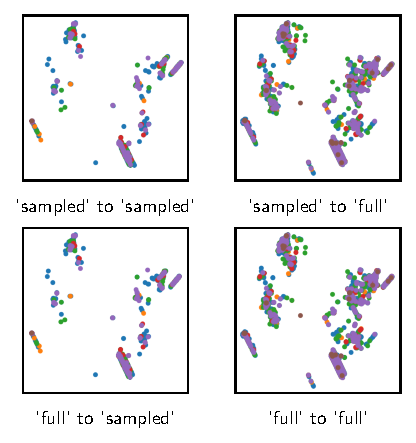
\includegraphics[width=.7\linewidth]{figures/pca-projection.pdf}
% 				\caption{Cross-projection of the malicious traffic from two datasets in two dimensions using PCA.}
% 			\end{figure}}
% 		\end{column}
% 	\end{columns}

% \end{frame}



\begin{frame}
\frametitle{Experimental setup}
\begin{itemize}
	\item Dataset:
	\begin{itemize}
		\item \textbf{sampled} NF-V2 version of CSE-CIC-IDS2018~\cite{sarhan_StandardFeatureSet_2022,sharafaldin_GeneratingNewIntrusion_2018}
		\item ports and IP addresses are removed
		\item 80\% for training, 20\% for testing (evenly distributed)
	\end{itemize}

	\only<2->{\item Model:
	\begin{itemize}
    \item \Acrfull{mlp} model with two hidden layers~\cite{popoola_FederatedDeepLearning_2021}
    \item Baseline (centralized training): F1-score of 0.966, accuracy of 0.992
	\end{itemize}}

	\only<3->{\item FL setup:
	\begin{itemize}
			\item Cross-silo setting: all clients are available at each round
			\item The dataset is partitioned into 10 \gls{iid} shards of 80,000 data points
			\item Models are aggregated using \texttt{FedAvg}
	\end{itemize}}

\end{itemize}
\end{frame}
\glsunset{mlp}


\section{Results}

\begin{frame}
	\frametitle{Impact predictability}
	\begin{itemize}
		\item Very high variance in the results
		\item The impact of the attack is highly dependent on the seed
		\begin{itemize}
			\item[$\rightarrow$] Initial parameters, data shuffling, \dots
		\end{itemize}
		\item Results tend to stabilize after a few rounds on different values
	\end{itemize}
	
	\vspace{\baselineskip}

	\begin{figure}
		\centering
		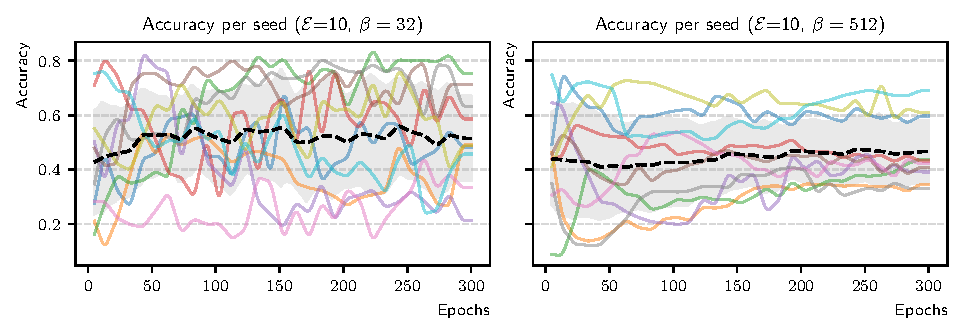
\includegraphics[width=.8\textwidth]{figures/predictability-all.pdf}
		\vspace{-2ex}
		\caption{Accuracy of the poisoned model by seed (50\% attackers).}
	\end{figure}
	
\end{frame}

\begin{frame}
	\frametitle{Hyperparameter influence}

	\begin{itemize}
		\item No impact on the average performance
		\item Significant impact on the variance of the results, but not really on convergence
	\end{itemize}

	\vspace{\baselineskip}

	\begin{figure}
		\centering
		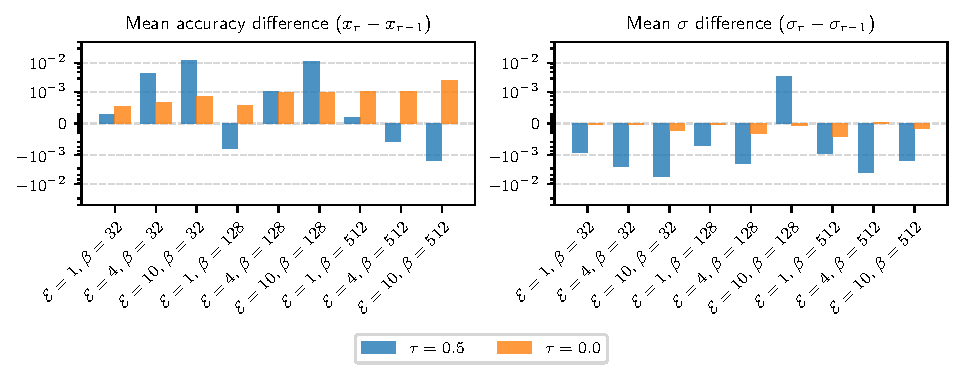
\includegraphics[width=.8\textwidth]{figures/hyperparams-continous-cicids-small.pdf}
		\vspace{-2ex}
		\caption{Effect of the hyperparameters on the accuracy of the poisoned model.}
	\end{figure}
\end{frame}

\begin{frame}
	\frametitle{Hyperparameter influence}

	\begin{itemize}
		\item \texttt{late-3} scenario: attackers start poisoning after 3 rounds
		\item High batch size leads to more inertia
		\begin{itemize}
			\item The impact is less instantaneous $\rightarrow$ more impactful in constrained environments
		\end{itemize}
	\end{itemize}

	\begin{figure}
		\centering
		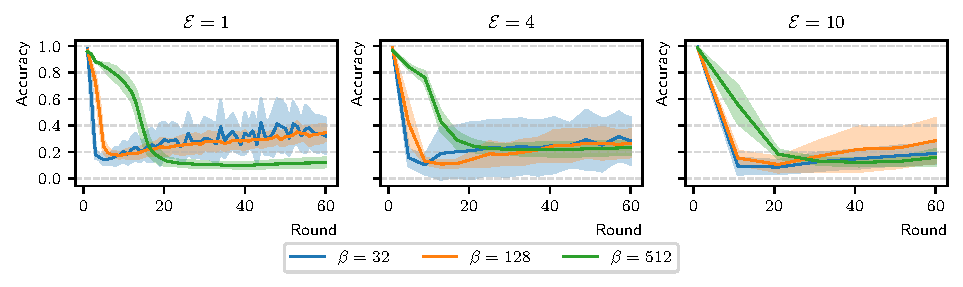
\includegraphics[width=\textwidth]{figures/hyperparams-late.pdf}
		\vspace{-2ex}
		\begin{minipage}{.7\textwidth}
			\caption{Effect of the hyperparameters on the accuracy of the poisoned model in the \texttt{late} scenario (50\% attackers).}
		\end{minipage}
	\end{figure}
\end{frame}

\begin{frame}

	\frametitle{Targeted attacks}
	\begin{figure}
		\centering
		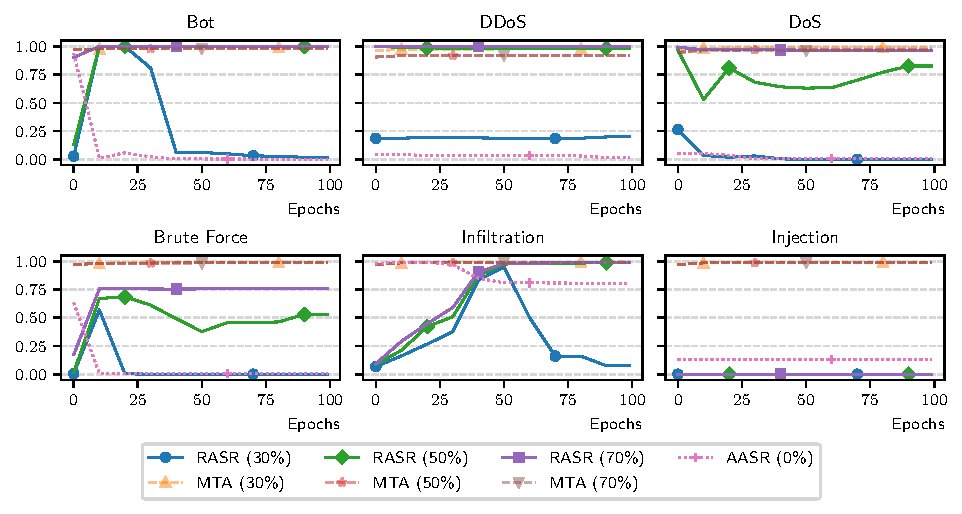
\includegraphics[width=.8\textwidth]{figures/backdoors.pdf}
		\caption{Backdoor success rate.}
	\end{figure}

\end{frame}

\begin{frame}
\frametitle{Targeted attacks}

Can we build an IDS backdoor using label-flipping?
\begin{itemize}
	\item Yes, but\dots\only<2>{
	\item The model's generalization capabilities can mitigate the impact
	\begin{itemize}
		\item especially with characteristic overlaps between classes
	\end{itemize}
	\item The attack's effectiveness is highly dependent on the target
	\item We need a significant number of attackers.
	}
\end{itemize}
\end{frame}


\section{Conclusion}

\begin{frame}
\frametitle{Conclusion}

\begin{itemize}
	\item A \emph{reproducible evaluation framework} to study the impact of label-flipping attacks in \gls{fids} using \gls{fl}.
	\begin{itemize}
		\item reproducible, extendable, and available in open-access
		\item first step towards a more comprehensive evaluation and comparison of poisoning attacks and their mitigation strategies.
	\end{itemize}
	\vspace{1ex}
	\item A \emph{deeper understanding of the behavior of label-flipping attacks} in FL-based CIDSs.
	\begin{itemize}
		\item The behavior of poisoning attacks is unpredictable.
		\item It is dependent on the hyperparameters, but not on the average performance.
		\item Targeted attacks can be effective but are highly dependent on the model's generalization capabilities.
	\end{itemize}
\end{itemize}
\centering\vspace{4\baselineskip}
$\rightarrow$ \small\emph{more detailed results in the paper :)}
\end{frame}




\begin{frame}
	\frametitle{Future Work}
	\begin{itemize}
		\item Extend the study to other datasets. \only<2>{\textcolor{red}{[DONE]}}
		\item Extend to other feature sets and poisoning attacks.
		\item Build more appropriate metrics for the evaluation of poisoning attacks in different data distributions.
		\item Study the impact of the data distribution on the ability to detect attacks using similarity metrics. \only<2>{\textcolor{red}{[DONE]}}
	\end{itemize}

	% \vspace{3\baselineskip}
	% \begin{center}
	% 	\only<2>{\emph{
	% 		Want to know about the new results? I defend my thesis on \textbf{October 7th, 2024} at \textbf{14:00} in \textbf{Rennes}. You are welcome to join!
	% 	}}
	% \end{center}
\end{frame}

\begin{frame}[allowframebreaks]
	\frametitle{References}
	\printbibliography
\end{frame}

\begin{frame}
	\frametitle{Thank you!}
	\vspace{1ex}

	\begin{itemize}
		\item Consider the use case when designing or choosing mitigations.
		\item Expect the unexpected: the behavior of poisoning attacks is unpredictable.
		\item Try it yourself! Our work is \emph{reproducible} and everything is in \emph{open-access}!
	\end{itemize}\vspace{2ex}

	\begin{columns}
		\hfil\hfil
		\begin{column}{.25\textwidth}
			\centering
			\small Paper\\
			
\includegraphics[width=.8\linewidth]{figures/qr-paper.png}
		\end{column}
		\hfil
		\begin{column}{.25\textwidth}
			\centering
			\small Results\\
			
\includegraphics[width=.8\linewidth]{figures/qr-results.png}
		\end{column}
		\hfil\hfil
		\begin{column}{.25\textwidth}
			\centering
			\small Evaluation framework\\
			
\includegraphics[width=.8\linewidth]{figures/qr-eiffel.png}
		\end{column}
	\end{columns}
	\vspace{4ex}
	\centering\Large Any questions?


\end{frame}

\section*{Appendix}

\begin{frame}
	\frametitle{Threat model implementation}

	\begin{itemize}
			\item A malicious participant can alter its local dataset before training, and start/stop the attack at any round $r$.
			\begin{itemize}
				\item Either done by the client itself or by an external attacker.
			\end{itemize}
			\item The attacker can manipulate labels of its dataset.
			\begin{itemize}
				\item Untargeted: flip the labels of a proportion of samples.
				\item Targeted: associate benign labels to a proportion of samples from a specific attack class.
			\end{itemize}
			\item An attacker can poison any proportion of its local data
			\begin{itemize}
				\item \Acrfull{dpr}: ($\alpha$) $\rightarrow$ proportion of flipped samples.
			\end{itemize}
			\item Multiple attackers can collude to perform the attack.
			\begin{itemize}
				\item \Acrfull{mpr}: ($\tau$) $\rightarrow$ proportion of attackers.
			\end{itemize}
	\end{itemize}
\end{frame}
\glsunset{dpr}
\glsunset{mpr}

\begin{frame}
	\frametitle{RQ3: Can FL heal itself from poisoning attacks?}
	\begin{figure}
		\centering
		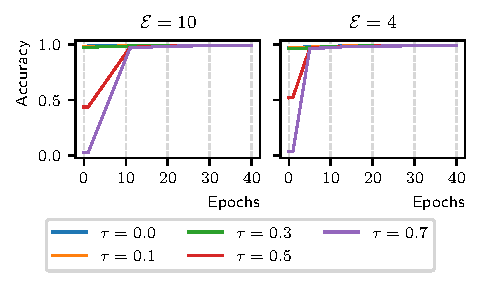
\includegraphics[width=.5\textwidth]{figures/redemption.pdf}
		\caption{Recovery of the model after a poisoning attack.}
	\end{figure}
\end{frame}

\begin{frame}
	\frametitle{RQ5: Is there a critical threshold for label-flipping to be effective?}

	\vspace{-2ex}
	\begin{figure}
		\centering
		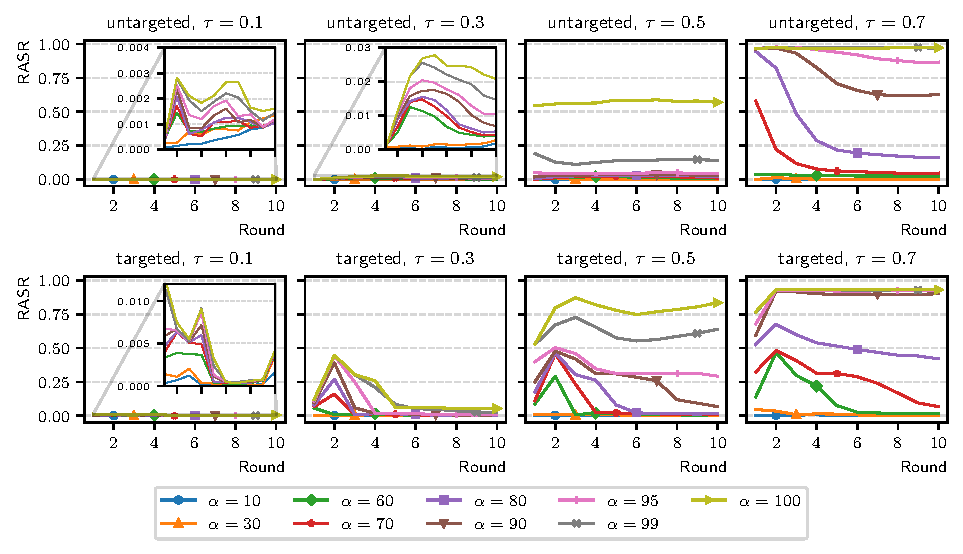
\includegraphics[width=.8\textwidth]{figures/attacks.pdf}
		\vspace{-2ex}
		\caption{Impact of $\tau$ and $\alpha$ on the attack's effectiveness.}
	\end{figure}

\end{frame}
	
\end{document}